\subsection{分析}

将1月23日至4月23日所有天的业务量时间序列按月汇总作图. 从图中可以看出个别天的数据很异常, 查日历知道2017年1月27日是除夕夜, 从实际因素分析, 本文推断可能是除夕前人们需要准备送礼或准备压岁钱ATM机导致交易量增加, 春节期间人们走亲访友导致交易量减少, 因此决定分段处理日总交易. 而不同日期的业务量峰值变化很大, 尤其是1月27日前业务量的峰值明显高于其他日期的业务量峰值. 1月27日后几天, 业务量峰值又明显小于其他日期. 除夕当天业务量从上午到下午有一个缓慢降低的过程. 这一点可从春节前人们大量购买年货, 春节后进入假期, 人们很少购物来解释.

\begin{figure}[H]
    \centering
    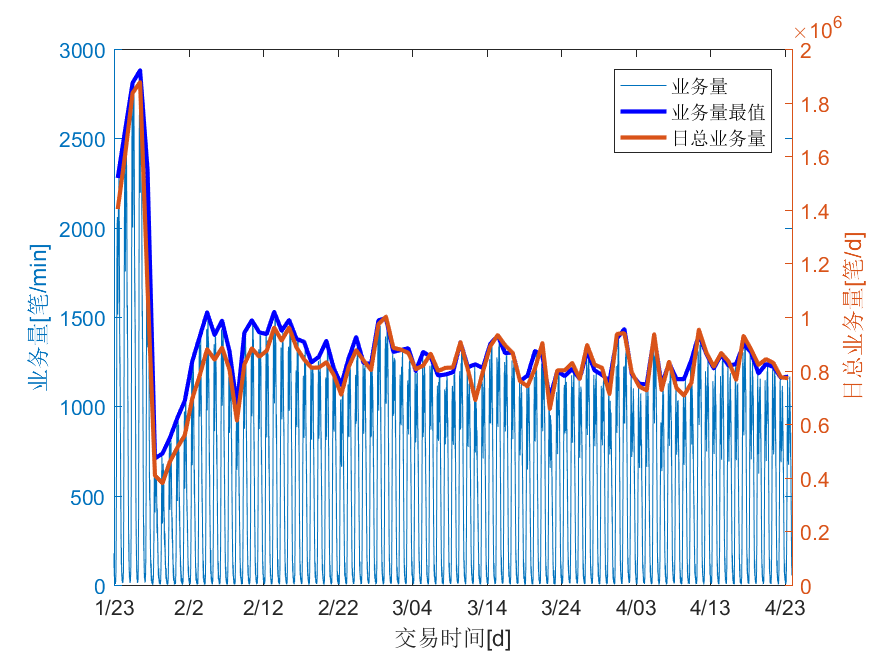
\includegraphics[width=7cm]{lr1.png}
    \caption{交易量随日期的变化}
\end{figure}

而在春节之后, 本文发现每日交易总量并没有明显的以七天为周期的变化规律. 因而难以发现其中工作日和休息日的交易变化区别. 为了简化问题, 所以本文假定工作日和非工作日的交易量不存在明显差别.

另外, 从上图中可以看出: 在1月23日至1月27日, 1月28日至2月1日的日平均交易量存在明显差别. 为了更加明显表示其区别, 本文在一张图上表示出这三段时间的平均交易量随时间的变化.

\begin{figure}[H]
    \centering
    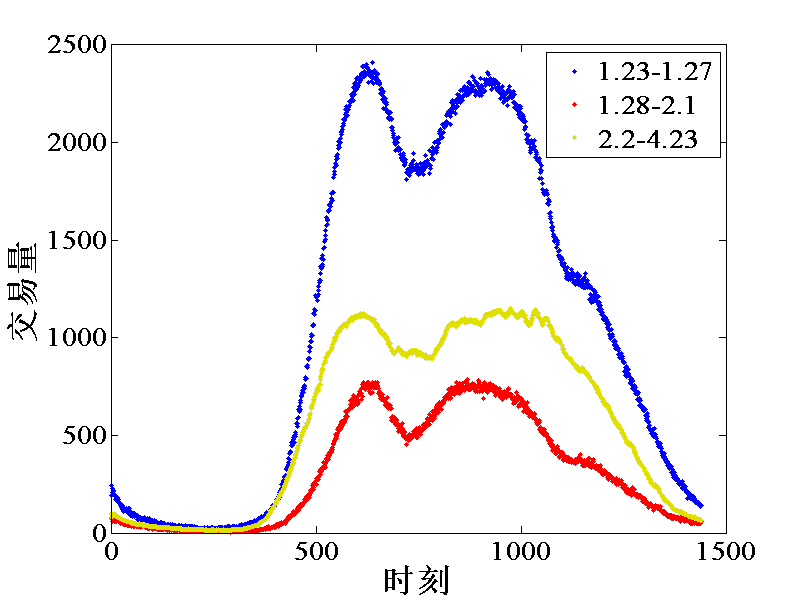
\includegraphics[width=7cm]{lr2.png}
    \caption{三段时间内平均交易量在一天各时刻的变化}
\end{figure}

由每日交易量随时间的变化图可知, 交易量在早晚各有一个高峰. 交易量的主要特征体现在早晚两个高峰中, 对交易量分布的分析也需要从这早晚两个高峰入手. 考虑到现实意义和模型的可操作性, 本文认为交易量在早晚高峰期分别满足满足两种不同的正态分布, 而总的交易分布, 应是这两个正态分布的合分布. 对于这种多参多峰的复杂分布, 在求解参数时, 为了使拟合分布与实际数据有着很好的贴合度, 本文打算利用EM算法来求双峰高斯函数的参数.

\subsection{特征参数选取}

EM算法分为两步: E(expectation)步, 求隐变量的期望.M(maximum)步, 求似然函数的最大值. 具体应用到多元高斯模型中, M步需要求解
\begin{figure}[H]
    \centering
    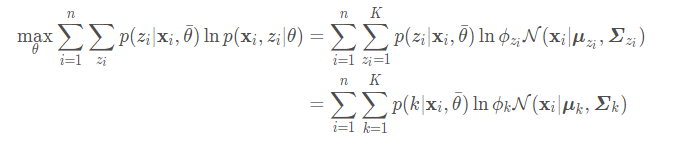
\includegraphics[width=14cm]{lr3.png}
\end{figure}

注意到$p(k|\vect{x}_{i}, \bar{\theta})$不包含优化变量$\theta$, 因此在此问题中可以看作关于$i$和$k$的常数, 故我们暂记其为$\gamma_{ik}$, 留到最后再讨论其具体取值. 忽略掉优化无关常数, M步的优化问题正式写作:
\begin{figure}[H]
    \centering
    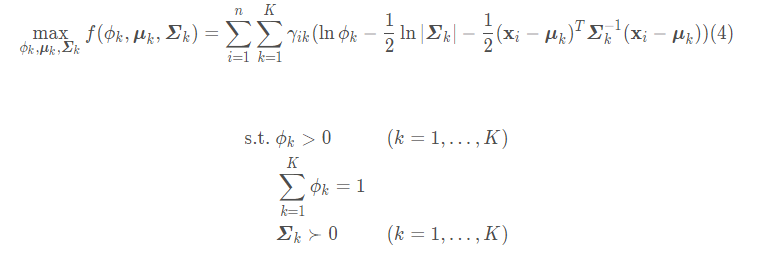
\includegraphics[width=14cm]{lr4.png}
\end{figure}

综上所述, 可得整个算法如下:
\begin{figure}[H]
    \centering
    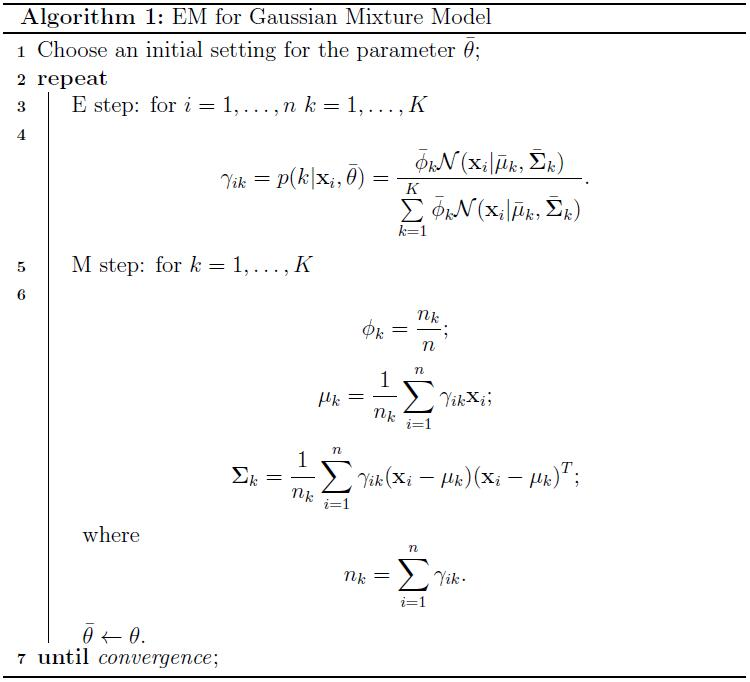
\includegraphics[width=14cm]{lr5.png}
\end{figure}

进行拟合求解后, 本文得到如下结果(以1月25日为例):

\begin{figure}[H]
    \begin{minipage}[b]{0.49\textwidth}
        \centering
        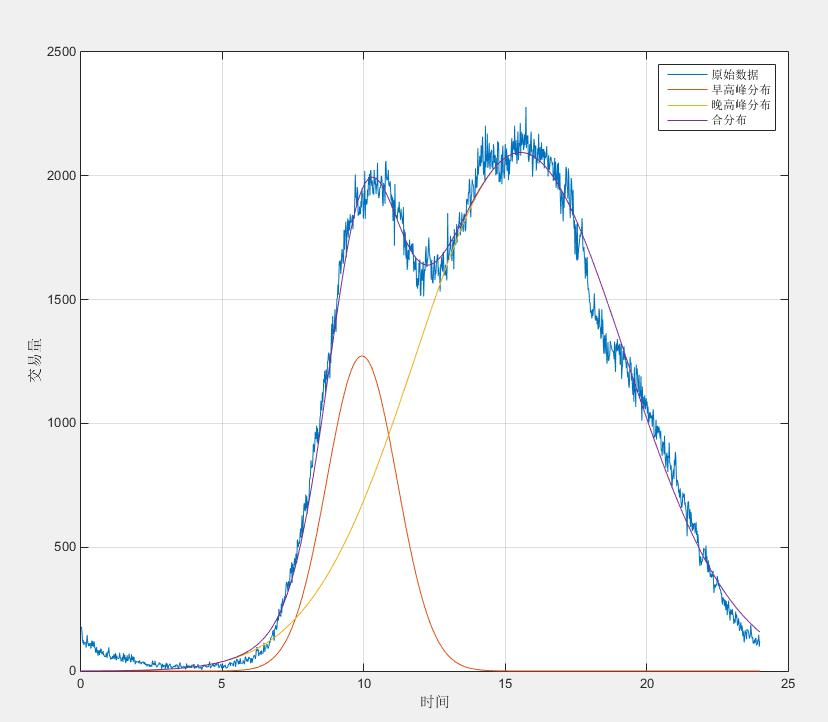
\includegraphics[width=7cm]{lr6.png}
        \captionof{figure}{1月25日交易量随时间分布拟合图像}
    \end{minipage}
    \hfill
    \begin{minipage}[b]{0.49\textwidth}
        \centering
        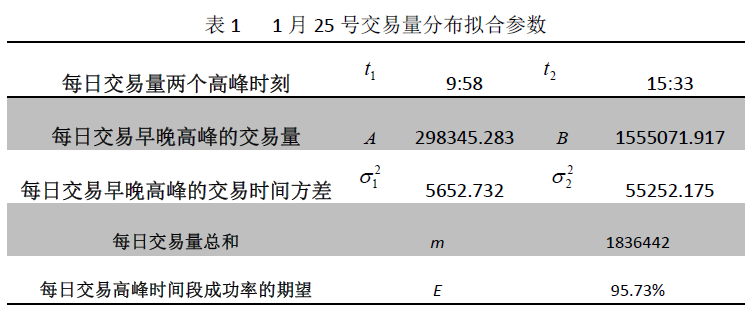
\includegraphics[width=7cm]{lr7.png}
        \captionof{figure}{1月25日交易量随时间分布拟合参数}
    \end{minipage}
\end{figure}
